\section{Sampling proposals}\label{app:sampling}

Figure~\ref{fig:appendix-mcmc-traj} provides a schematic of molecular graph evolution under \gls{mcmc}
steps for \gls{gem} on QM9 and MOSES.

\begin{figure*}[h]
\centering
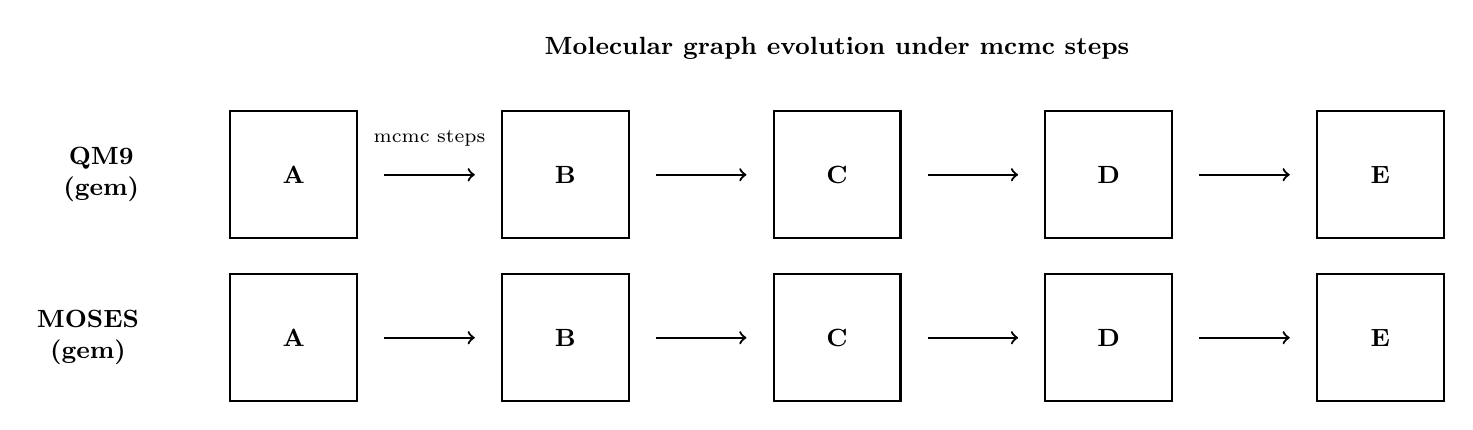
\begin{tikzpicture}[scale=1.15]
  % Layout constants
  \def\boxsize{1.4}
  \def\gap{3.0}
  \def\rowgap{1.8}
  \def\arrowlen{1.0}

  \pgfmathsetmacro{\titlex}{2*\gap + 0.5*\boxsize}
  \node[font=\small\bfseries] at (\titlex,2.1) {Molecular graph evolution under \gls{mcmc} steps};

  % Row labels
  \node[anchor=east, align=center, font=\small\bfseries] at (-0.9,0.5*\boxsize) {QM9\\(\gls{gem})};
  \node[anchor=east, align=center, font=\small\bfseries] at (-0.9,-\rowgap+0.5*\boxsize) {MOSES\\(\gls{gem})};

  % Row 1 (QM9)
  \foreach \i/\lab in {0/A,1/B,2/C,3/D,4/E} {
    \draw[thick] (\i*\gap,0) rectangle ++(\boxsize,\boxsize);
    \node[font=\small\bfseries] at (\i*\gap+0.5*\boxsize,0.5*\boxsize) {\lab};
  }
  \foreach \i in {0,1,2,3} {
    \draw[->, thick]
      ({\i*\gap + 0.5*(\gap+\boxsize) - 0.5*\arrowlen}, {0.5*\boxsize})
      -- ({\i*\gap + 0.5*(\gap+\boxsize) + 0.5*\arrowlen}, {0.5*\boxsize});
  }
  \node[font=\scriptsize] at ({0.5*(\gap+\boxsize)}, {0.5*\boxsize+0.4}) {\gls{mcmc} steps};

  % Row 2 (MOSES)
  \foreach \i/\lab in {0/A,1/B,2/C,3/D,4/E} {
    \draw[thick] (\i*\gap,-\rowgap) rectangle ++(\boxsize,\boxsize);
    \node[font=\small\bfseries] at (\i*\gap+0.5*\boxsize,-\rowgap+0.5*\boxsize) {\lab};
  }
  \foreach \i in {0,1,2,3} {
    \draw[->, thick]
      ({\i*\gap + 0.5*(\gap+\boxsize) - 0.5*\arrowlen}, {-\rowgap+0.5*\boxsize})
      -- ({\i*\gap + 0.5*(\gap+\boxsize) + 0.5*\arrowlen}, {-\rowgap+0.5*\boxsize});
  }
\end{tikzpicture}
\caption{\footnotesize \textbf{\gls{mcmc} Evolution.} Molecular graph evolution under \gls{mcmc} steps for \gls{gem} on QM9 and MOSES. \textcolor{red}{[WiP]}}
\label{fig:appendix-mcmc-traj}
\end{figure*}
